\documentclass[a4paper,11pt]{article}

\usepackage{acl-ijcnlp2009}

\usepackage{epsfig} \usepackage{times} \usepackage{url} \usepackage{latexsym}

\title{Self Organizing Maps in a Learning Game}

\author{Keith Stevens \\ University of California, Los Angeles \\
kstevens@cs.ucla.edu}

\date{}

\begin{document}

\maketitle

\section{Introduction}
%hypothesis goes here, apprach, claims and goals also go here.
Acquiring the first aspects of language in artificial agents is a problem that
has been addressed by a variety of approaches.  There are symbolic approachs
which use logical inferences to deduce which object a word refers too
\cite{Siskind}, and approaches which use simple decision trees and predicate
logic to ground the meaning of a word \cite{GoldNico}.  There are also
statistical approaches which utilize bayesian statistics to compute the
likelihood of a word grounding to a particular object based on it's usage
\cite{FazlyProbRefUn,SmithCommSystem,VogtSocial}.  Each of these approachs have
worked to tackle a central issue, the presence of referential uncertainty.  

Referential uncertainty is a term describing the situation where a word can be
heard, and several objects could be present to a young learning agent.  The
agent would then have to decide which object the word most likely refers too.
This is best described by Quine \cite{Quine} with his "gavagi" problem, where an
anthropologist is traveling with a tribe of people speaking a foreign tongue,
and suddenly one of them points to a rabbit and speaks "gavagi".  Knowing no
words for this language so far, the antrhopologist must guess which object the
word refers to, usually by observing multiple uses of the word, in different
contexts.  Both symbolic and stastitical approachs have relied on the key
assumption that words are eventually used in enough contexts to clarify their
meaning.

Recently, a connectionist model has been introduced which models early word
acquisition by use of several connected self organizing maps
\cite{LiDevLex,MiikDisLex}.  This system has the appealing ability to model a
growing lexicon, which can be challenging in connectionist systems due to
catastrophic interference, by training connections between the two maps with
pairs of semantic representations and phonological representations.  One issue
mentioned by the authors earlier in \cite{FarkasWcd} is that connectionist
systems tend to learn based of unrealistic data, and address this problem by
taking incorporating word co-occurance information into the semantic
representations based on the agents current lexicon.  The one key feature
missing from this system is the incorporation of referential uncertainty when
learning.

This project introduces a combination of a simplified version of the DevLex
architecture \cite{LiDevLex}, and a simple learning game frequently uesd for
bootstraping lexical groundings in stastistical agents
\cite{VogtLearningSim,VogtSocial}.  There are two key initial challenges in this
project.  First, can agents using self organizing maps correctly agree on a
language when no language currently exists when there is no referential
uncertainty?  Second, can these agents, or an enhancement of these agents,
handle referential uncertainty when learning?

\section{Overview and the Learning Game}
%describe the hypotheses in more detail.
A simulation of how humans acquire their first words would present a situation
where an agent which a well defined lexicon speaks about the world with a new
agent, but this well estabilished agent would have to be designed by hand.  As
such, approximation of early word acquisition has been used which allows new
agents to bootstrap their lexicons through simple learning games
\cite{VogtLearningSim,VogtSocial}.  In some resepects, this approximation is
similar to young children interacting in a world with objects they are not
familiar with.  

\begin{figure} \center 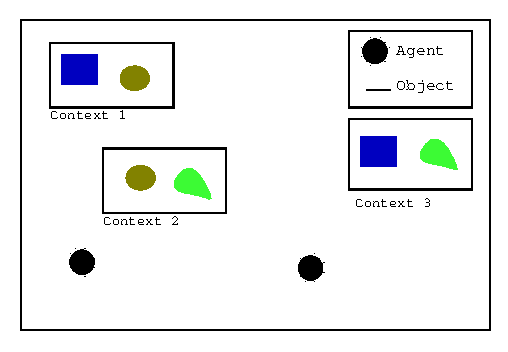
\includegraphics[width=.49\textwidth]{game-env.eps}
\caption{Sample game environment with 2 agents.} \label{fig:game-env}
\end{figure}

Each learning game have the following basic steps:

\begin{enumerate}

\item A speaker is choosen.

\item A speaker choose a set of objects to speak about.  It then choose on of
the objects within the context to be the focus object of the learning game.

\item The speaker speaks some word which best describes the focus object.

\item The hearer learns to accociate the spoken word with the focus object.

\end{enumerate}

There are three basic versions of a simple learning game introduced in
\cite{VogtLearningSim}, which are each progressively more difficult to handle.

\begin{enumerate}

\item Observation Game: Speakers inform the hearer of the focus object before
speaking.

\item Guessing Game: The hearer is not informed of the focus object, but can
point to the object it gusses to be the focus object, and the speaker can either
confirm or correct the guess.

\item Selfish Game: The hearer is not informed of the focus object, and makes no
response during the learning game.

\end{enumerate}

The Observation Game is of little interest for this project since this is akin
to telepathicly telling each agent what the mapping should be, and side steps
the presence of referential uncertainty altogether.  The Guessing Game is of
some interest, since this represents either correction or a reward after making
a guess.  The last version of the learning game, the Selfish Game, is of the
most interest, since if the speaker has a well defined lexicon, this would be a
close simulation of a parent speaking about the world, with a child passively
overhearing the conversation and attempting to map the words to present objects.
In the current model of bootstraping lexicon, it still is of interest, as it
could be considered to be a simulation of a child observing two other children
speaking with each other.

One key issue in both games is deciding when each the speaker and hearer should
learn a mapping from a word to an observation.  The speaker will always have an
advantage because the focus object is known to the agent, so in both game types,
the speaker can learn a mapping as soon as a word is produced for the focus
object.  The hearer on the other hand has a different time of learning based on
the game type.  In the Guessing game, learning should take place after the agent
guesses what the focus object is, and receives some feed back.  In the Selfish
Game, the agent has only one option for learning, the time of observation.

It is my main hypotheses is that a simple self organizing map should be
sufficent for a small population of agents to agree on a small artificial
language without referential uncertainty using on the Selfish Game.  Once
referential uncertainty in introduced, the self organizing map alone will be
insufficent, and would need some additional mechanism, yet should still be
feasible with the Selfish Game.

\section{Architecture}

%archetecture goes here, along with description of software packages used, and
%the current status of each module.
In order to accomodate multiple experiments, the connectionist architecture has
a simple, modular design.  There are two standard Self Organizing Maps, one for
semantic representations, and one for phonological representations, where all
nodes in one map are connected to all nodes in the other map.  Each neuron in
the two haps has meaning vector, and an activation associatted with it.  Each
connection between nodes from the semantic and phonological map has a
uni-directional weight.  Each map also monotonically decreases the size of the
neighboorhod over time.  Additionally, each neuron in the semantic map has a set
of attentional weights which will vary based on variation of semantic meanings
mapped to the particular neuron.  Figure \ref{fig:arch} provides a graphical
description of this architecture.

\begin{figure} \center 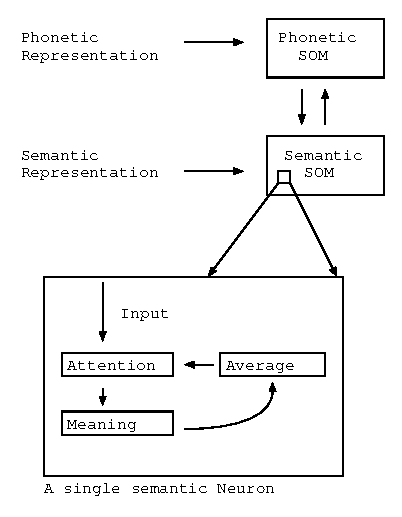
\includegraphics[width=.49\textwidth]{arch.eps}
\caption{Architecture of a single learning agent} \label{fig:arch} \end{figure}

Aside from the attentional weights maintained for each neuron, the basic
structure of the two self organizing maps is derived from
\cite{LiDevLex,MiikDisLex}, and is summarized as follows.

When a new input stimuluse, $x$ is presented to the map for training, a winning
neuron is found by finding the neuron $k$ whose meaning vector, $m_k$ has the
smallest euclidian distance to $x$.  Neuron $k$ will then be the central of all
updates done to the map, with $N_k$ being the set of neighboors to $m_k$.  The
meaning vector of each neuron in a map, is then updated according to the a
slight modification to the standard SOM update scheme:

{\small \begin{equation}\label{eq:meaning_weight}
m_{ij}(t+1) = m_{ij}(t) + N(i)*\alpha(t)[atten_{ij}(t)x_j - m_{ij}(t)]
\end{equation} }

where $N(i)$ is 1 if node $i \in N_c$ and 0 otherwise, $\alpha(t)$ is the
learning weight which decreases monotonically, and $atten_{ij}(t)$ is the
attentional weight of each feature in a semantic representation, and defined as

\begin{equation}\label{eq:atten}
att_{ij}(t) = 1 / (1 + variance_{ij})
\end{equation}

The variance of each feature is maintained as a rolling variance, along with a
rolling average based on the techniques presented in
\cite{mints93rollingvariance}.

To maintain the unidirectional link between nodes of each map, the activation of
each node must first be computed, where the highest activation will be centered
around the winning node, and a spread of activation within the node's
neighboorhod is produced in each map.  Formally, this activation is computed as:

\begin{equation}\label{eq:act}
a_i = N(i)*(1 - \frac{||\textbf{x} - \textbf{m$_i$}|| - d_{min} }{d_{max} -
d_{min}})
\end{equation}

where $d_{min}$ and $d_{max}$ are the smallest and largest meaning distances
within $N_c$.  With these activations, the uni-directional hebbian weights are
updated with:

\begin{equation}\label{eq:heb_weight}
w_{kl}(t+1) = w_{kl}(t) + \alpha(t+1)a_k^Sa_l^D
\end{equation}

which maintains a two dimensional matrix of weights, and is then normalized
according to row length normalization.  When training, a string representation
of the word is also presented to the system.  When phonlogical representations
are present, the word is mapped to the winning node in the phonlogical map.
Otherwise, the word is mapped to the winning node in the semantic map.

For production, a winning node is produced in the map which recieves input by
again selecting the node whose meaning vector has the smallest euclidian
distance to the input $x$.  The activation for the nodes in this map are againt
computed using Equation \ref{eq:act}.  The activations in the output map are
produced by propogaing the source activation over the hebbian links using:

\begin{equation}\label{eq:prop}
a_l^D = \sum_k w_{kl}a_k^S
\end{equation}

And the output produced by the output map is decided by the node which has the
highest activation.

Lastly, the neighboorhood $N_k$ is defined by

\begin{equation}\label{eq:neighboors}
N_k = \{ i \:| \:|| \textbf{loc$_i$} - \textbf{loc$_k$} || \leq 50\exp(\frac
{-t}{177})\}
\end{equation}

\subsection{Configurations to the system}

Since several configurations of learning need to be tested, several of the
components can be disconnected and turned off.  The attentional weights can be
shut off completely, simply by initializing all weights to 1 and not using
Equation \ref{eq:atten}.  Similarly, phonological mappings can be shut off by
ignoreing Equaltions \ref{eq:act}, \ref{eq:heb_weight} and \ref{eq:prop}.  In
this configuration, production is simply done by producing the word mapped to
the winning node in the semantic map.

\section{Input}

\begin{center}
  \begin{table*}
    \begin{tabular}[t] { | l | c | c | }
      \hline
      Word & Category & Vector \\
      \hline
      ball & Toys & \includegraphics[width=.80\textwidth]{ball.ppm} \\
      cheese & Food \& Drink & \includegraphics[width=.80\textwidth]{cheese.ppm} \\
      juice & Food \& Drink &\includegraphics[width=.80\textwidth]{juice.ppm} \\ 
      milk & Food \& Drink &\includegraphics[width=.80\textwidth]{milk.ppm} \\ 
      pants & Clothing & \includegraphics[width=.80\textwidth]{pants.ppm} \\
      sock & Clothing &\includegraphics[width=.80\textwidth]{sock.ppm} \\
      \hline
    \end{tabular}
    \caption{Sample vectors for semantic representations}
    \label{tb:semantics}
  \end{table*}
\end{center}

%general io and specific examples goes here.
Two forms of input need to be fed into the system, semantic representations and
phonological representations.  Additionally there is a fixed lexicon of words
which is accompanied by the phonological representations.  For phonetics,
vectors produced from the PatPho system \cite{LiPatPho}.  These vectors have 15
real valued features which are produced based on how each word fits into a
syllable template.  PatPho vectors for 401 chinese words are used with the
pinyin romanization for the string form of each word.  A sample of these vectors
can be seen in Figure \ref{fig:phono}

The semantic vectors correspond to the objects placed in the learning environment.
For these semantic representations, initially 60 vectors, each with 60 real valued
features, were randomly generated.  In each random vector, 3 randome features were
randomly assigned a value between 0 and 1.  These random vectors had no underlying
patterns within them.

The other set of semantic vectors built using a feature generation system
\cite{HarmWordNetFeature}.  This feature generatin system first builds binary
features for the provided words based on information in the WordNet taxonomy.
Since these binary feature vectors are of a high dimension, they are reduced
using random mapping, the same process is used for the semantic vectors used in
\cite{LiDevLex}.  The 60 words used for generating vectors were taken from the
vocabulary from the MacArthur–Bates Communicative Development Inventories (CDI) \cite{DaleCDI}.
This list is a collection of words learned by toddlers in early stages of word
acquisition.  The 60 words selected were the first 60 in this list when sorted
according to age the word is acquired, and thus the earliest words acquired by
toddlers.  These words are approximately the first 60 words used in \cite{LiDevLex}.

\begin{figure} \center \includegraphics[width=.49\textwidth]{phono-gray.eps}
\caption{Gray scale vector of 6 sample phonological vectors.} \label{fig:phono} \end{figure}

\section{Experiment and result}
%describe the results
For this project, the experiment is to run a series of learning games with a
small number of learning agents to determine wether or not a population of simple connectionist
agents can agree on a language.  Several configurations of agents are run:

{\small
\begin{enumerate}

\item Agents use only a semantic map, with no attentional learning.

\item Agents use only a semantic map with attentional learning.

\item Agents ues both maps with no attentional learning.

\item Agents use both maps with attentional learning.

\end{enumerate}
}

In addition to these configurations for agents, the learning environment is
also moddifed to either include contexts in learning games, or not include
contexts (and thus reduce the difficulty in learning).

To evaluate each configuration, two key metrics are used.  First is language
convergens, monitoring how many objects all the agents are able to agree on a
single term.  Second is the rate of homonymy, measuring how many objects are
refered to by each word.  If both convergence and homonym are high, then the
agents have developed a vague and unusable language.  The ideal language should
have high convergence and low homonymy.  


\section{Discussion and conclusion}
%discuss the results, how they reflect on previous word, and what issues exist,
%and conclude.
some text here.  \bibliographystyle{acl} \bibliography{report}

\end{document}
